\documentclass[10pt,a4paper]{article}

\usepackage[left=1cm,right=1cm,top=1.5cm,bottom=1.5cm]{geometry}
\usepackage{amsmath,amssymb,amsfonts}
\usepackage{graphicx}
\usepackage{booktabs}
\usepackage{hyperref}
\usepackage{natbib}
\usepackage{xcolor}
\usepackage{multirow}
\usepackage{caption}
\usepackage{subcaption}
\usepackage{algorithm}
\usepackage{algpseudocode}

\newcommand{\cmark}{\checkmark}

\hypersetup{colorlinks=true, linkcolor=blue, citecolor=blue, urlcolor=blue}

\title{\textbf{Transformer's Revenge: Stress-Testing minGRU's Claims Against Attention on Algorithmic Reasoning Tasks}}

\author{
  Mayukh Das \quad Vibhansh Gupta \quad Daniel Vaz \quad Adam Clark
}

\date{COMP6242 Deep Learning, Semester 1, 2026}

\begin{document}
\maketitle

\begin{abstract}
\citet{feng2024were} recently asked ``Were RNNs All We Needed?'', showing that a minimal gated recurrent unit (minGRU) matches Transformer performance on standard language modelling benchmarks with $O(T)$ complexity. We stress-test this claim by moving beyond language modelling into tasks requiring explicit algorithmic reasoning (verbatim sequence copying and induction head pattern completion) where architectural limitations are exposed rather than masked by statistical regularity. In a controlled setting (${\sim}$750--800K parameter target, identical optimiser and schedule), we compare minGRU against a Transformer with RoPE and RMSNorm, and a causal gMLP architecture we adapt as a third paradigm bridging fixed-parameter spatial mixing and learned attention. Our 27-experiment grid ($3$ models $\times$ $3$ tasks $\times$ $3$ sequence lengths) demonstrates that minGRU's input-only gating fundamentally prevents content-based retrieval at \emph{any} sequence length, while gMLP succeeds within its fixed spatial window but fails beyond it. The Transformer remains the only architecture capable of unbounded algorithmic reasoning within training budget. We additionally observe a sharp phase transition in Transformer copy learning, consistent with recent work on circuit formation.
\end{abstract}

\section{Introduction}

\citet{feng2024were} make a provocative claim: by stripping the GRU to its minimal form and enabling parallel training via log-space scans, the resulting minGRU matches Transformer performance on language modelling while offering $O(T)$ linear complexity. Their experiments (character-level Shakespeare, a selective copying task, and reinforcement learning locomotion) support this claim within those domains. But language modelling primarily tests statistical pattern learning from local context, a setting where even simple $n$-gram models perform surprisingly well. The question we ask is: \emph{does the claim hold when we move beyond statistical modelling into tasks requiring explicit algorithmic reasoning?}

We engage directly with the minGRU paper by reproducing their architecture in a controlled setting and then subjecting it to tasks specifically designed to test capabilities that the architectural analysis suggests should be impossible. Our experimental design is a stress test: we already suspect where minGRU will fail based on its mathematical structure, but we verify this empirically and precisely characterise the failure boundaries.

To contextualise minGRU's capabilities, we compare against two architectures:

\begin{itemize}
    \item \textbf{A nanoGPT-based Transformer} enhanced with key LLaMA-recipe modifications \citep{touvron2023llama}: RoPE \citep{su2024roformer} for relative position encoding and RMSNorm \citep{zhang2019root} for stable pre-norm residuals, with all biases removed. We use GELU rather than SwiGLU for the FFN activation, as SwiGLU's benefits are less pronounced at small model scales and we observed training instability at this parameter budget in prior coursework (COMP8650 AML). This represents the attention-based upper bound.
    \item \textbf{A causal gMLP} \citep{liu2021pay}: Our contribution adapting the originally bidirectional gMLP for autoregressive generation as a third paradigm. The gMLP uses fixed spatial weights rather than data-dependent attention, placing it architecturally \emph{between} the minGRU (no cross-position interaction beyond recurrence) and the Transformer (full data-dependent cross-position interaction). This allows us to disentangle \emph{whether} a model can mix across positions from \emph{how} it mixes.
\end{itemize}

All models use 4 layers; the theoretical and empirical justification for this depth choice is discussed in Section~\ref{sec:model_config}.

We test on three tasks of increasing algorithmic difficulty: character-level language modelling (TinyShakespeare), verbatim sequence copying, and induction head pattern completion, each at three sequence lengths chosen to cross architectural boundaries. This yields a $3 \times 3 \times 3 = 27$ experiment grid from which we derive predictions \emph{a priori} and then verify experimentally.

\section{Background and Architectural Analysis}

\subsection{Transformer with LLaMA-Inspired Modifications}

Our Transformer builds on the nanoGPT codebase, enhanced with key modifications from the LLaMA recipe \citep{touvron2023llama}: pre-norm residual connections using RMSNorm \citep{zhang2019root}, Rotary Position Embeddings (RoPE) \citep{su2024roformer}, and removal of all bias terms. The core mechanism is multi-head causal self-attention:
\begin{equation}
    \text{Attention}(Q, K, V) = \text{softmax}\left(\frac{QK^\top}{\sqrt{d_k}} + M\right)V
\end{equation}
where $M$ is a causal mask ($M_{ij} = -\infty$ for $j > i$). RoPE rotates query and key vectors by position-dependent angles, enabling attention scores to depend only on relative distance $m - n$ without learned absolute embeddings.

\textbf{Key property}: Every token attends to \emph{every} preceding token with a learned, \emph{content-dependent} weight. The attention matrix provides unbounded context access; the only constraint is $O(T^2)$ compute cost.

\subsection{minGRU: The Claim Under Test}

The minGRU \citep{feng2024were} strips the classical GRU to its minimal form, removing the reset gate entirely and enabling parallel training via log-space cumulative sums:
\begin{align}
    g_t &= \sigma(W_g x_t + b_g) \label{eq:mingru_gate} \\
    \tilde{h}_t &= W_h x_t + b_h \\
    h_t &= (1 - g_t) \odot h_{t-1} + g_t \odot \tilde{h}_t
\end{align}

The parallel form computes all hidden states simultaneously:
\begin{equation}
    \log h_t = \text{logcumsumexp}\left(\sum_{k=1}^{t} \log(1-g_k),\; \log g_t + \log \tilde{h}_t\right)
\end{equation}

This achieves $O(T)$ complexity and enables efficient GPU utilisation through parallel scan operations. \citet{feng2024were} demonstrate competitive perplexity on language modelling benchmarks, motivating their claim.

\textbf{Critical limitation}: The gate $g_t$ in Eq.~\ref{eq:mingru_gate} depends \emph{only on the current input} $x_t$, not on the hidden state $h_{t-1}$, not on any future query about what to retrieve. The model must decide at write-time what to store, without knowledge of what will be needed later. For tasks requiring content-based retrieval (``find the token that appeared after $A$''), this is architecturally insufficient: the gate cannot implement a selective read operation conditioned on a query. This is the specific weakness we target in our stress test.

\subsection{Causal gMLP: A Third Paradigm (Our Contribution)}

We adapt the originally \emph{bidirectional} gMLP architecture \citep{liu2021pay} for autoregressive generation as a third comparison point. The original gMLP was proposed for classification tasks using full $T \times T$ spatial projections; we modify it with causal masking and a windowed SGU for efficient generation. The gMLP replaces attention with a Spatial Gating Unit (SGU) that applies a learned linear projection across the sequence dimension:
\begin{align}
    U, V &= \text{split}(\text{Linear}(x)) \\
    V' &= (W_s V + b_s) \quad \text{where } W_s \in \mathbb{R}^{T \times T} \\
    \text{SGU}(x) &= U \odot V'
\end{align}

For causal modelling, $W_s$ is masked to be lower-triangular. We restrict $W_s$ to a banded structure with window size $w = 256$:
\begin{equation}
    (W_s)_{ij} = \begin{cases} w_{ij} & \text{if } 0 \leq i - j < w \\ 0 & \text{otherwise} \end{cases}
\end{equation}

The gMLP occupies a unique position in our comparison: unlike minGRU, it \emph{does} perform explicit cross-position information mixing. Unlike the Transformer, this mixing uses \emph{fixed} parameters rather than content-dependent queries. This disentangles two questions: (1) can the model route information across positions at all? (2) can it do so in a content-dependent manner?

\textbf{Critical limitation}: The spatial weights $W_s$ are fixed parameters: token $t$ aggregates from $[t{-}w{+}1, \ldots, t]$ with weights independent of content. Beyond window $w$, information is inaccessible in a single layer. While $L$ layers give a theoretical receptive field of $L \times w$, precise token-level retrieval beyond one window is impractical.

\subsection{A Priori Predictions}

From the architectural analysis above, we derive three predictions before running experiments:

\begin{enumerate}
    \item \textbf{Transformer}: should succeed on all tasks. Attention provides unbounded, content-dependent access to all prior tokens; no architectural barrier exists for copy or induction at any length.
    \item \textbf{minGRU}: will fail on all algorithmic tasks regardless of sequence length. Input-only gating (Eq.~\ref{eq:mingru_gate}) cannot implement content-based retrieval; this is a structural impossibility, not a capacity issue.
    \item \textbf{gMLP}: will succeed on algorithmic tasks where the required retrieval distance falls within its 256-token window, and fail beyond it. The boundary should be sharp, not gradual.
\end{enumerate}

All three models should achieve comparable performance on Shakespeare, since language modelling relies on local statistical patterns, precisely the domain where \citet{feng2024were} demonstrated parity. The algorithmic tasks, by contrast, require \emph{exact} content-based retrieval across arbitrary distances, which directly tests the architectural limitations identified above.

\section{Experimental Setup}

\subsection{Tasks and Data}

\textbf{TinyShakespeare.} Character-level language modelling on the 1.1M-character Shakespeare corpus (65-character vocabulary). We use a 90/10 train/validation split. This directly mirrors the type of benchmark on which \citet{feng2024were} demonstrated minGRU's competitiveness. Metric: validation perplexity.

\textbf{Long-Range Copy.} Sequences of the form \texttt{[content][separator][content]}, where the model must reproduce the first half verbatim after the separator. Content is drawn from a 26-character alphabet. Short: $T{=}128$ (64 tokens to memorise), Medium: $T{=}528$ (256 tokens), Long: $T{=}2048$ (1024 tokens). This task requires pure storage and retrieval; no statistical shortcut exists. Metric: recall perplexity (computed only on the recalled portion).

\textbf{Induction Heads.} Sequences containing repeated bigram patterns: after observing $[A][B]$ earlier in the sequence, the model must predict $B$ when $A$ reappears. Generated at $T \in \{128, 256, 2048\}$ with 5 induction patterns per sequence. This tests content-based retrieval: the model must use the current token $A$ as a \emph{query} to find what followed $A$ previously. Metric: masked accuracy on induction positions only.

\subsection{Model Configurations}

\label{sec:model_config}
All models use 4 layers with hidden dimension 128, targeting ${\sim}$750--800K parameters:

\begin{table}[h]
\centering
\caption{Model configurations. All share 4 layers and $d{=}128$.}
\small
\begin{tabular}{lccc}
\toprule
 & \textbf{Transformer} & \textbf{gMLP} & \textbf{minGRU} \\
\midrule
Parameters & ${\sim}$795K & ${\sim}$508--933K\textsuperscript{$*$} & ${\sim}$737K \\
Layers & 4 & 4 & 4 \\
Hidden dim & 128 & 128 & 128 \\
Attention/Window & 4 heads & $w{=}256$ & -- \\
FFN & GELU, $4 \times d$ & GELU, $d_\text{ffn}{=}512$ & GELU, $4.5 \times d$ \\
Normalisation & RMSNorm & LayerNorm & RMSNorm \\
Position encoding & RoPE & Learned & Implicit (recurrence) \\
Additional & bias=False & -- & Conv1d ($k{=}4$) \\
\bottomrule
\end{tabular}

{\footnotesize \textsuperscript{$*$}gMLP parameter count varies with sequence length due to the $T \times T$ spatial weight matrix within the SGU.}
\end{table}

The depth of 4 layers is motivated by theoretical results showing exponential expressiveness gains from depth \citep{telgarsky2016benefits}: deeper networks can represent functions requiring exponentially more parameters in shallower architectures. The hierarchical composition enabled by depth \citep{bengio2011shallow, montufar2014number} is particularly important for our algorithmic tasks, where multi-step reasoning (identify pattern, locate match, retrieve next token) benefits from layered processing. Our depth choice aligns with \citeauthor{feng2024were}'s finding that 3 layers are required for even simple memory tasks (1-layer achieves only 37\% on selective copy vs.\ 99.5\% at 3 layers).

\subsection{Training Protocol}

All 27 experiments share an identical training protocol to ensure fair comparison:
\begin{itemize}
    \item Optimiser: AdamW ($\beta_1{=}0.9$, $\beta_2{=}0.95$, weight decay $0.1$)
    \item Learning rate: cosine decay from $3 \times 10^{-4}$ to $3 \times 10^{-5}$
    \item Warmup: 200 steps (linear)
    \item Dropout: 0.05
    \item Gradient clipping: max norm 1.0
    \item Batch size: 64 (reduced to 32 for gMLP at $T{=}2048$ due to $O(T^2)$ memory)
    \item Steps: 5,000 for Shakespeare and Copy; 20,000 for Induction
    \item Hardware: NVIDIA A100 GPU (Google Colab)
\end{itemize}

\subsection{Implementation}

The minGRU implementation directly follows \citet{feng2024were}, reproducing their Appendix C.2 language modelling recipe: each block consists of a causal Conv1d ($k{=}4$), the minGRU cell, and an MLP, all with pre-norm RMSNorm and residual connections. The Transformer is built from nanoGPT with LLaMA-inspired modifications (RoPE, RMSNorm, no bias), reflecting a subset of the recipe validated at scale \citep{touvron2023llama}. The causal gMLP adapts \citet{liu2021pay} with a banded causal SGU (window $w{=}256$), as described in Section~2.3. Each model has an independent training script with shared interfaces for task specification. Data generation for synthetic tasks uses identical random processes across models. Source code is available at [repository link].

\section{Results}

\subsection{Overview}

Figure~\ref{fig:heatmap} presents the complete 27-experiment summary. The central finding is immediately visible: all models achieve comparable language modelling performance (confirming \citeauthor{feng2024were}'s claim in that domain), but algorithmic tasks expose sharp architectural boundaries that the language modelling evaluation entirely misses.

\begin{figure}[h]
    \centering
    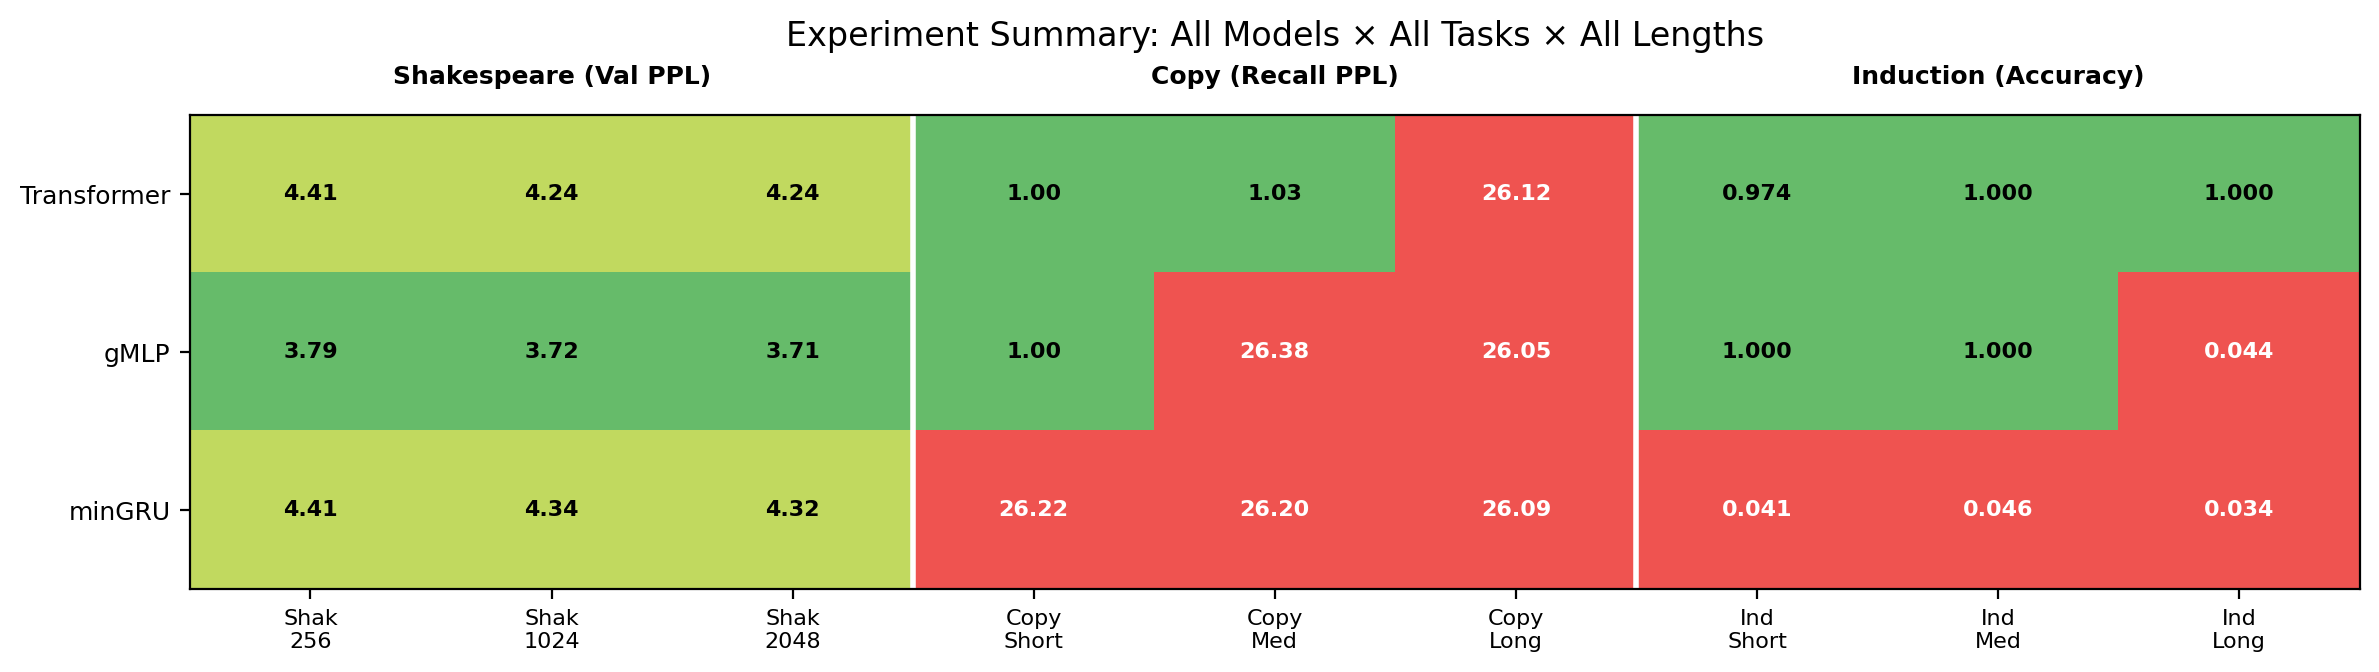
\includegraphics[width=\textwidth]{figures/07_summary_heatmap.png}
    \caption{Summary of all 27 experiments. Shakespeare: validation perplexity (lower = better). Copy: recall perplexity (1.0 = perfect, ${\sim}$26 = random). Induction: masked accuracy (1.0 = perfect, ${\sim}$0.04 = random). Colour: green = pass, yellow = partial, red = fail.}
    \label{fig:heatmap}
\end{figure}

\subsection{Stress Test: Algorithmic Tasks}

Figure~\ref{fig:algorithmic} shows performance as a function of sequence length for both algorithmic tasks, the core of our stress test.

\begin{figure}[h]
    \centering
    \begin{subfigure}[b]{0.48\textwidth}
        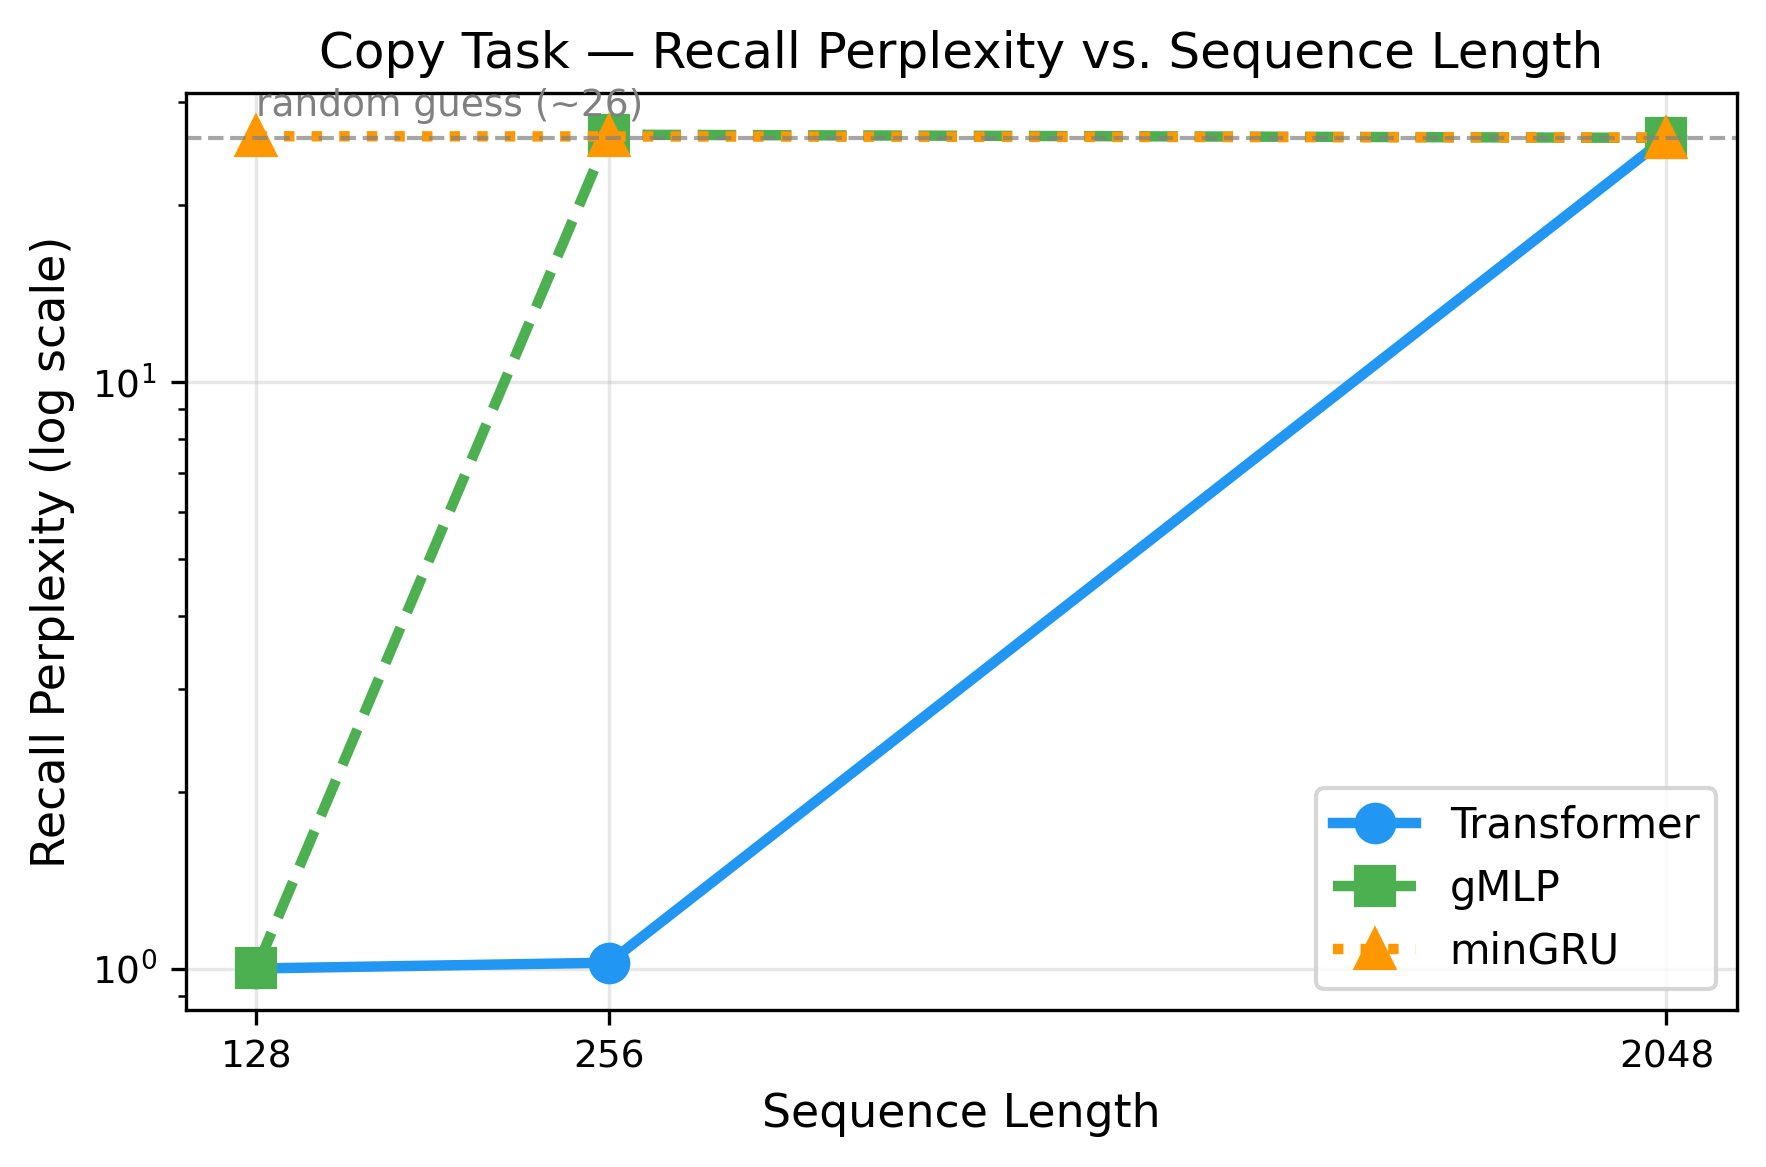
\includegraphics[width=\textwidth]{figures/fig1_copy_ppl_line.png}
        \caption{Copy task: recall perplexity (log scale).}
        \label{fig:copy}
    \end{subfigure}
    \hfill
    \begin{subfigure}[b]{0.48\textwidth}
        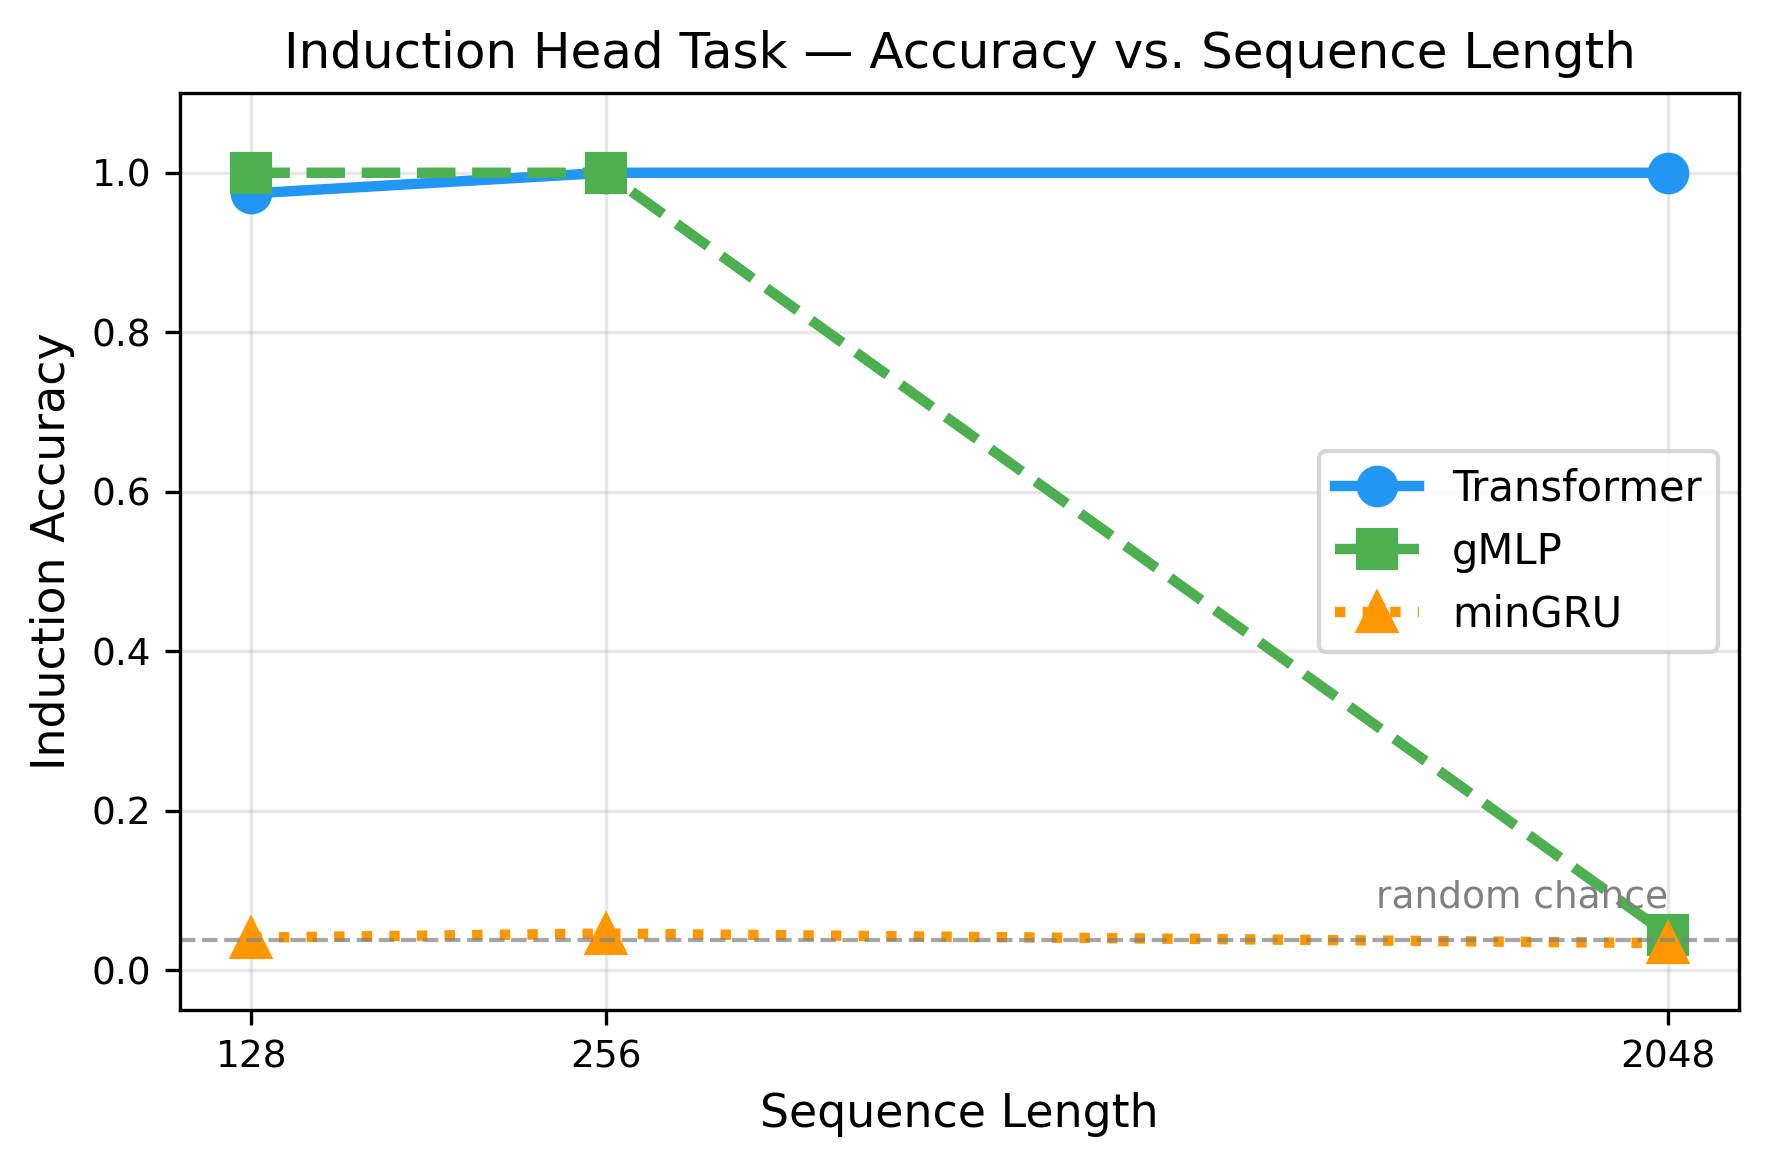
\includegraphics[width=\textwidth]{figures/fig2_induction_accuracy_line.png}
        \caption{Induction task: masked accuracy.}
        \label{fig:induction}
    \end{subfigure}
    \caption{Algorithmic task performance vs.\ sequence length. Each model's failure point maps precisely to its architectural limitation: minGRU fails at all lengths (no content-based retrieval), gMLP fails beyond its 256-token window, Transformer succeeds except where training budget is insufficient.}
    \label{fig:algorithmic}
\end{figure}

\textbf{Copy task} (Figure~\ref{fig:copy}): The Transformer achieves near-perfect recall (PPL ${\approx}1.0$) at short and medium lengths but fails at $T{=}2048$ (PPL $= 26.12$, equivalent to random). The gMLP succeeds at $T{=}128$ (within window) but fails at $T{=}528$ where the recall span exceeds its 256-token boundary. The minGRU fails at \emph{all} lengths (PPL ${\approx}26$), confirming that the limitation is architectural, not capacity-related.

\textbf{Induction task} (Figure~\ref{fig:induction}): The Transformer achieves ${\geq}0.97$ accuracy at all lengths. The gMLP matches this at $T{=}128$ and $T{=}256$ (within window) but collapses to random chance ($0.044$) at $T{=}2048$. The minGRU achieves only random-chance accuracy (${\approx}0.04$) regardless of sequence length; it cannot implement the ``query by content'' operation that induction requires.

\textbf{Key result}: \citeauthor{feng2024were}'s claim that minGRU is competitive with Transformers holds strictly for statistical language modelling but \emph{categorically fails} for algorithmic reasoning tasks. The failure is not due to insufficient capacity or training; it is a fundamental architectural limitation of input-only gating.

\subsection{Confirming the Claim: Language Modelling}

\begin{figure}[h]
    \centering
    \begin{subfigure}[b]{0.48\textwidth}
        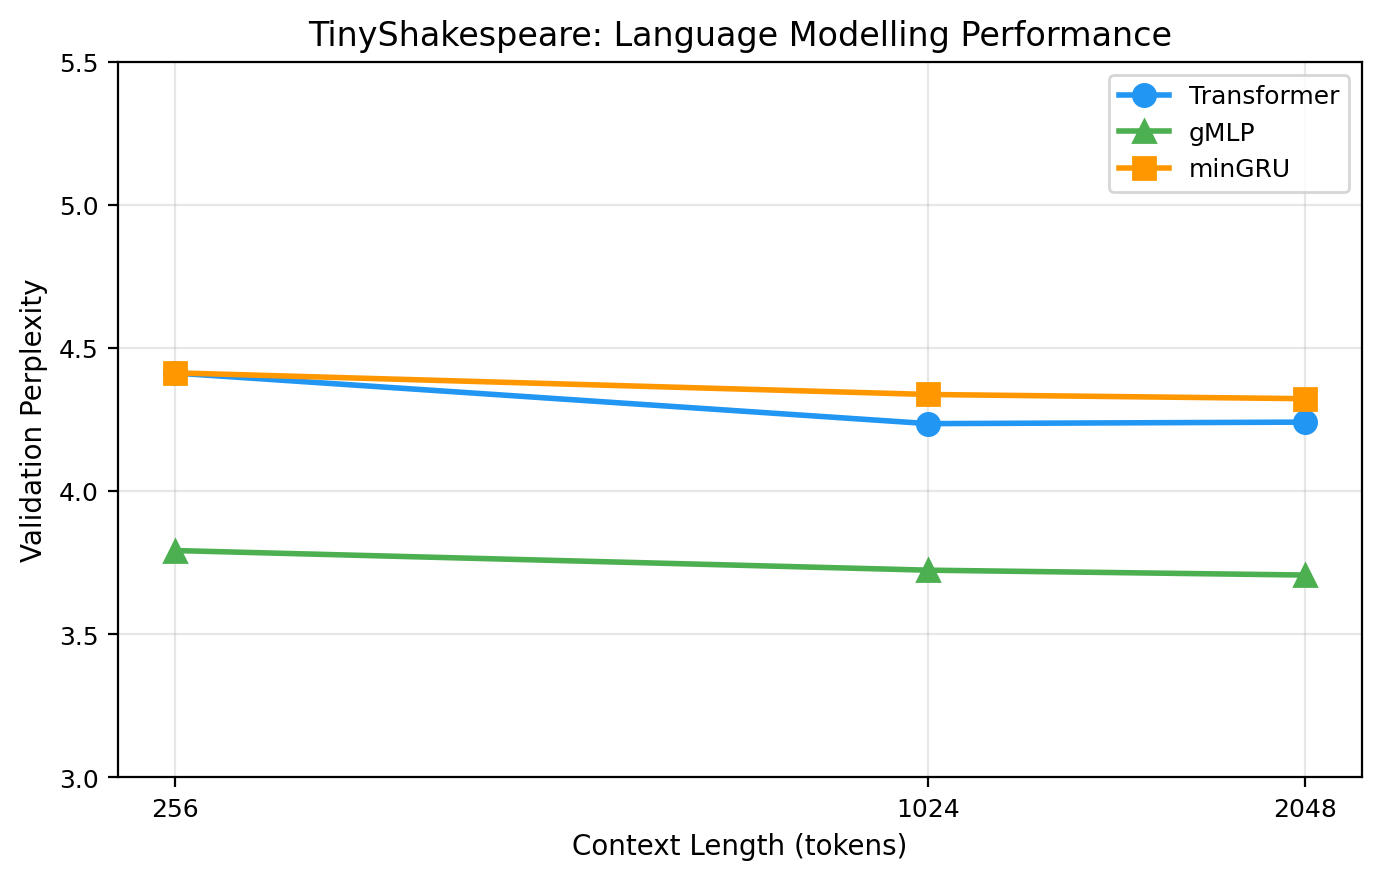
\includegraphics[width=\textwidth]{figures/03_shakespeare_ppl.png}
        \caption{TinyShakespeare validation perplexity.}
        \label{fig:shakespeare}
    \end{subfigure}
    \hfill
    \begin{subfigure}[b]{0.48\textwidth}
        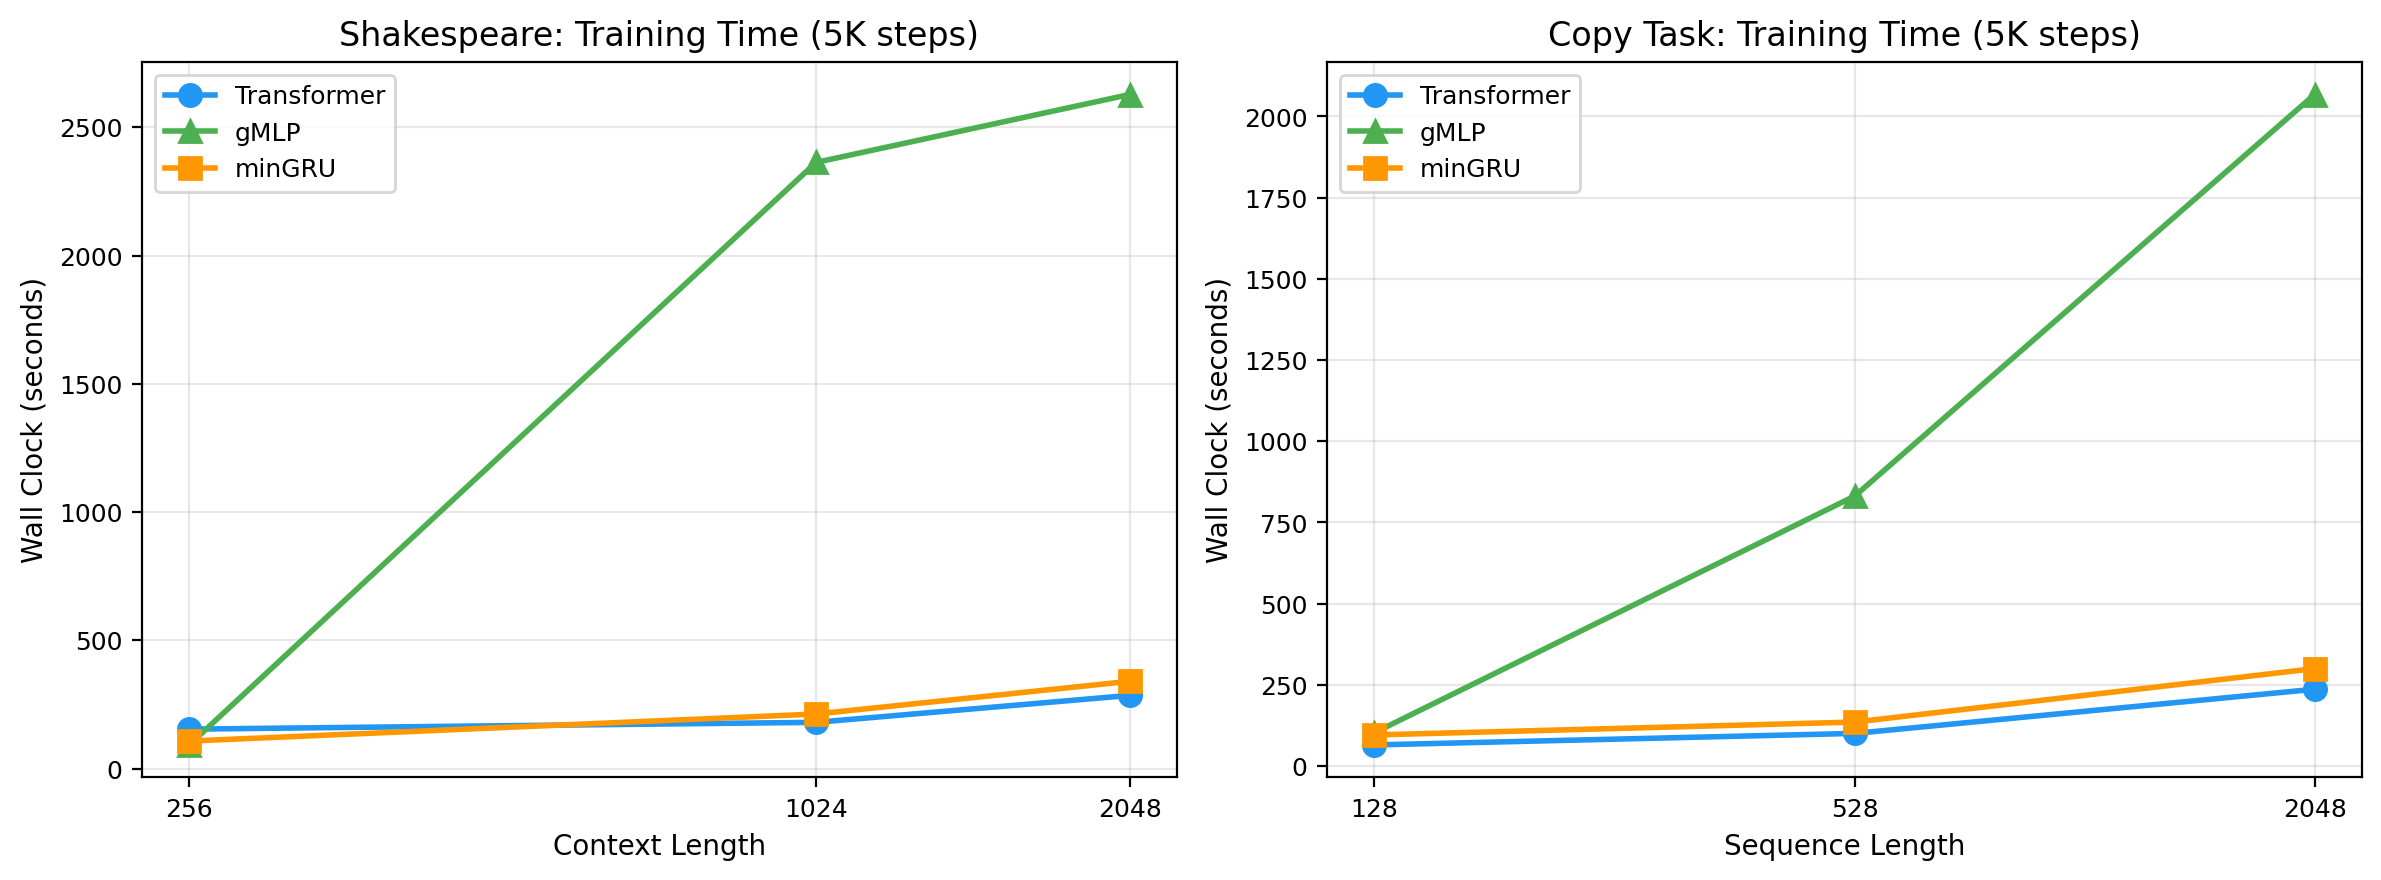
\includegraphics[width=\textwidth]{figures/04_wall_clock.png}
        \caption{Wall-clock training time vs.\ sequence length.}
        \label{fig:wallclock}
    \end{subfigure}
    \caption{(a) All models achieve comparable language modelling perplexity, confirming \citeauthor{feng2024were}'s claim in that domain. (b) Wall-clock training time. Transformer benefits from optimised GPU kernels; minGRU scales most gently; gMLP is slowest at long sequences.}
\end{figure}

On TinyShakespeare (Figure~\ref{fig:shakespeare}), all three architectures achieve similar perplexity (3.7--4.4), confirming \citeauthor{feng2024were}'s central result. In their own experiments, the Transformer achieves validation loss 1.547 versus minGRU's 1.548, near-identical parity that our results mirror. The gMLP achieves the lowest perplexity (3.71), consistent with natural language being predominantly local. These results validate that the algorithmic task failures are not artefacts of implementation quality or insufficient model capacity.

Figure~\ref{fig:wallclock} shows wall-clock training time. The Transformer is fastest overall, benefiting from highly optimised GPU attention implementations in PyTorch. minGRU's $O(T)$ parallel scan shows the gentlest growth with sequence length, suggesting it would overtake the Transformer at longer sequences where $O(T^2)$ attention becomes dominant. The gMLP is slowest at long sequences due to its unoptimised $T \times T$ spatial matrix, requiring batch size reduction to 32 at $T{=}2048$ to fit in memory.

\subsection{Phase Transition: Evidence of Circuit Formation}

\begin{figure}[h]
    \centering
    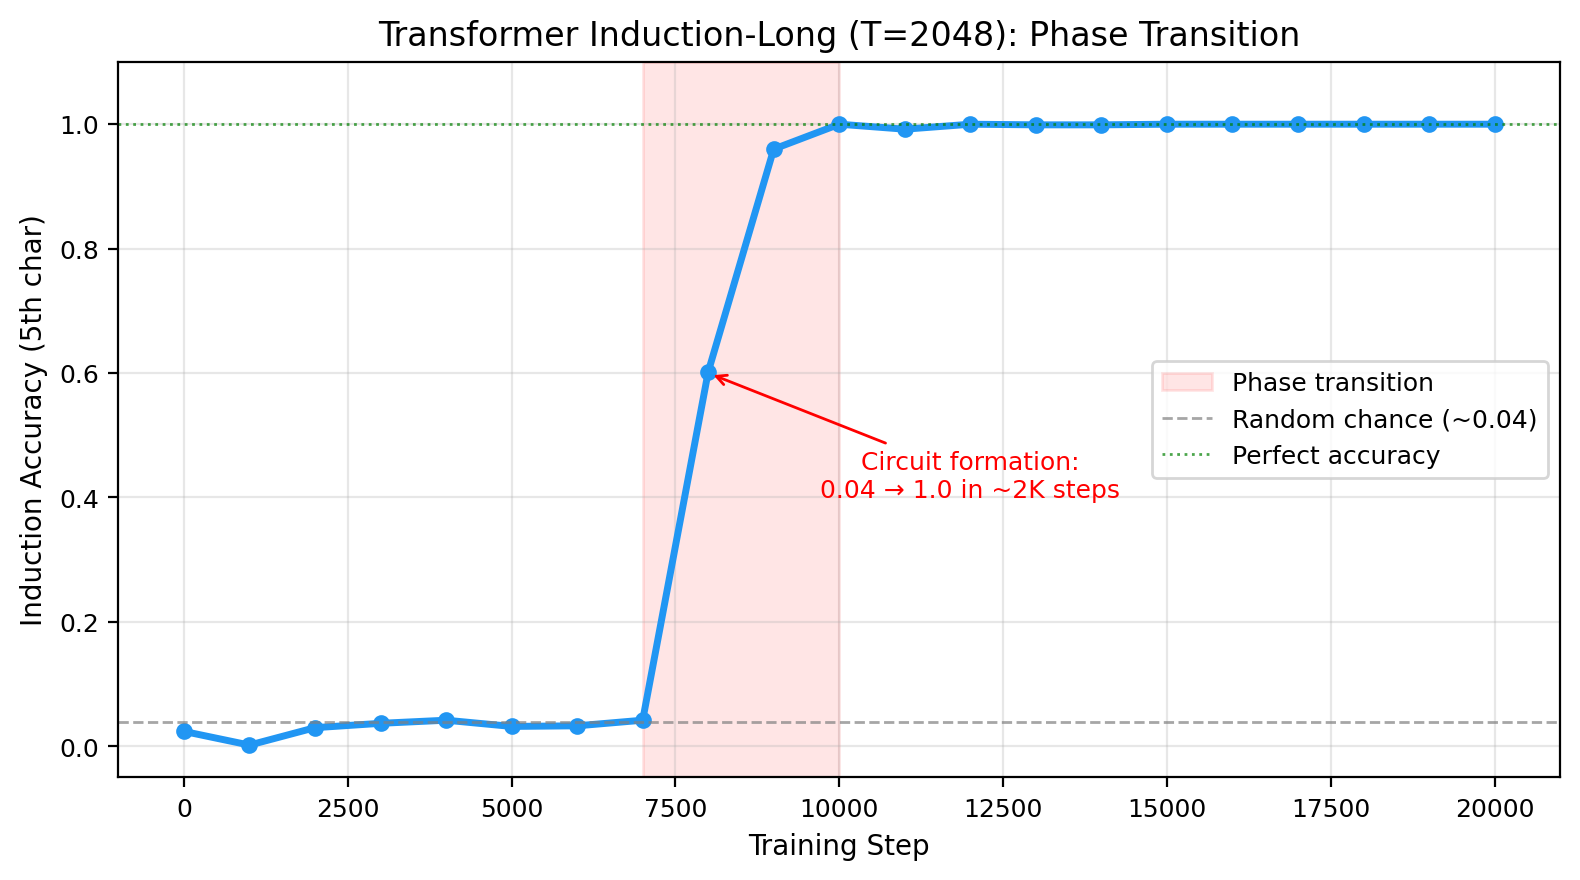
\includegraphics[width=0.55\textwidth]{figures/06_phase_transition.png}
    \caption{Training dynamics for Transformer on induction-long ($T{=}2048$). The model remains at random chance (0.04) for 7,000 steps, then abruptly jumps to perfect accuracy within 2,000 steps.}
    \label{fig:phase}
\end{figure}

Figure~\ref{fig:phase} reveals a striking training dynamic: the Transformer's induction-long accuracy remains at random baseline (0.04) for 7,000 steps, then undergoes a rapid phase transition to perfect accuracy (1.0) within ${\sim}$2,000 steps. This is consistent with ``grokking'' \citep{power2022grokking} and the circuit formation hypothesis \citep{olsson2022context}: the attention heads abruptly snap into an induction circuit configuration. This implies the Transformer's failure at $T{=}2048$ copy likely reflects insufficient training (5K steps) for the phase transition to occur, rather than an architectural limitation; given more steps, we predict the copy circuit would similarly emerge.

\section{Discussion}

\subsection{The Boundaries of ``Were RNNs All We Needed?''}

Our results precisely delineate where \citeauthor{feng2024were}'s claim holds and where it breaks:

\begin{itemize}
    \item \textbf{Claim holds}: For language modelling tasks dominated by local statistical patterns, minGRU is competitive with Transformers while being faster to train. Our Shakespeare results confirm this.
    \item \textbf{Claim breaks}: For any task requiring \emph{content-based retrieval} (using the current input as a query to selectively access past information), minGRU categorically fails. This is not a training or scale issue; it is a mathematical consequence of Eq.~\ref{eq:mingru_gate}.
\end{itemize}

The distinction maps to a concrete architectural criterion: does the task require \emph{data-dependent} information routing? If the answer is yes, input-only gating is insufficient.

It is important to distinguish our findings from \citeauthor{feng2024were}'s own ``selective copying'' experiment (adapted from \citealt{gu2023mamba}), where minGRU achieves 99.5\% accuracy. Their task is \emph{content-aware filtering}: certain tokens are marked as important at encoding time, and the model need only retain those marked tokens while ignoring distractors. This succeeds because the gate $g_t$ can learn to open for marked tokens; it is a \emph{write-time} decision. Our tasks are fundamentally harder: in verbatim copy, \emph{all} tokens must be stored; in induction heads, retrieval is conditioned on a future query (a \emph{read-time} decision). This is precisely the boundary that input-only gating cannot cross, as noted by \citet{merrill2024illusion} in their theoretical analysis of state-space expressiveness without state-dependent gating.

\subsection{Predictions vs.\ Reality}

Table~\ref{tab:comparison} compares our a priori predictions against observed outcomes:

\begin{table}[h]
\centering
\caption{Predicted vs.\ observed outcomes. All architectural predictions confirmed.}
\label{tab:comparison}
\small
\begin{tabular}{lccl}
\toprule
\textbf{Experiment} & \textbf{Predicted} & \textbf{Observed} & \textbf{Match} \\
\midrule
minGRU Copy (all lengths) & $\times$ & $\times$ (PPL $\approx$26) & \cmark \\
minGRU Induction (all) & $\times$ & $\times$ (Acc $\approx$0.04) & \cmark \\
gMLP Copy-Short & \checkmark & \checkmark\ (PPL=1.003) & \cmark \\
gMLP Copy-Medium & $\times$ & $\times$ (PPL=26.4) & \cmark \\
gMLP Induction-Long & $\times$ & $\times$ (Acc=0.044) & \cmark \\
Transformer Copy-Long & \checkmark & $\times$ (PPL=26.1) & $\times$\textsuperscript{$*$} \\
All Shakespeare & \checkmark & \checkmark & \cmark \\
\bottomrule
\end{tabular}
\end{table}

{\footnotesize \textsuperscript{$*$}Training budget limitation, not architectural (see Section 4.4).}

All predictions were confirmed except one: the Transformer failed on copy-long despite having no architectural barrier. The phase transition evidence (Section 4.4) explains this: the attention mechanism can solve the task but requires more than 5K steps to discover the circuit at $T{=}2048$. This is a training budget limitation, not an architectural one, and reinforces rather than undermines the core finding: only attention \emph{can} solve these tasks, even if it sometimes needs more time to do so.

One might argue our results reflect confirmation bias, that we chose tasks designed to expose failures. We contend the opposite: if the claim is that RNNs are ``all we needed,'' then the architecture should succeed on tasks the Transformer handles routinely. Induction heads and copy are not exotic benchmarks; they are fundamental capabilities that emerge naturally in trained Transformers \citep{olsson2022context}. A model that claims to replace Transformers must handle Transformer-native tasks.

\subsection{Implications: The gMLP Diagnostic and Architecture Selection}

The gMLP's role in our study is diagnostic: it answers whether cross-position mixing is sufficient, or must be content-dependent. Within its window, gMLP achieves perfect algorithmic performance: fixed spatial weights \emph{can} learn arbitrary routing over a bounded range. Beyond it, performance collapses discontinuously (not gradually), confirming a \emph{hard} boundary. This positions gMLP as architecturally intermediate: it has cross-position mixing (unlike minGRU) but not data-dependent mixing (unlike Transformer), confirming that the critical ingredient for unbounded algorithmic reasoning is content-dependent attention.

These findings yield actionable guidance: (1) for statistical/local tasks, minGRU is viable and efficient; (2) for bounded retrieval with known maximum distance, gMLP with window $\geq$ that distance suffices; (3) for unbounded or content-addressed retrieval, attention remains necessary.

\section{Limitations and Future Work}

\textbf{Parameter matching.} The gMLP's spatial weight matrix scales with $T$, making exact parameter matching across lengths impossible. At $T{=}2048$, gMLP has ${\sim}$933K parameters vs.\ ${\sim}$795K for others; this \emph{favours} gMLP, making its long-range failures more striking.

\textbf{Normalisation and position encoding.} Models use different normalisation (RMSNorm vs.\ LayerNorm) and position encoding (RoPE, learned, implicit). We follow each architecture's original specification rather than artificially unifying components. These differences are unlikely to explain pass/fail boundaries: both norms are mathematically similar at our scale, and position encoding differences would favour gMLP (exact learned positions) over the Transformer on copy tasks.

\textbf{Single seed.} All experiments use seed 42. While results are qualitatively unambiguous (pass/fail), multiple seeds would strengthen quantitative claims.

\textbf{Batch size.} gMLP at $T{=}2048$ uses batch size 32 (vs.\ 64) due to memory constraints, resulting in half the gradient samples per step.

\textbf{Future directions:}
\begin{itemize}
    \item Extend Transformer copy-long training beyond 5K steps to verify whether the phase transition eventually occurs (our analysis predicts it should).
    \item Compare with Mamba \citep{gu2023mamba}, which has \emph{state-dependent} gating; we predict it would overcome minGRU's limitation while retaining $O(T)$ complexity.
    \item Test minLSTM \citep{feng2024were}, which uses separate forget and input gates ($f_t$, $i_t$) providing a theoretically richer gating mechanism than minGRU's single gate. We chose minGRU over minLSTM for this study due to its superior training stability (\citeauthor{feng2024were} report variance up to $\pm 5.8\%$ for minLSTM vs.\ $\pm 0.2\%$ for minGRU); however, the separate gates may enable partial content-based retrieval that the single-gate minGRU cannot.
    \item Multi-seed experiments: our results are qualitatively unambiguous (pass/fail), but statistical confidence intervals would strengthen quantitative claims. Time budget constraints limited us to seed 42 across all 27 experiments.
    \item Attention head visualisation to confirm the hypothesised copy/induction circuit structure.
    \item Test hybrid architectures (gMLP + sparse global attention) to find the minimal attention needed for long-range capability.
\end{itemize}

\section{Conclusion}

Our 27-experiment stress test shows that \citeauthor{feng2024were}'s claim holds for statistical language modelling but categorically fails for algorithmic reasoning. The answer to ``were RNNs all we needed?'' is ``for which tasks?'', and the boundary is precisely whether the task requires data-dependent information routing. When it does, content-dependent attention remains necessary; no efficient alternative tested here can substitute.

\bibliographystyle{plainnat}
\bibliography{references}

\section*{Declaration}

\subsection*{Individual Contributions}
\begin{itemize}
    \item \textbf{Mayukh Das}, ID: u7965027: gMLP paper selection, experiment design, architecture comparison framework, implementation ideation, bug fixes (induction data generator, position mask, training protocol), report writing, presentation, paper review (Feng et al., gMLP)
    \item \textbf{Vibhansh Gupta}, ID: u7861976: Feng et al.\ paper selection, causal gMLP implementation, implementation ideation, presentation, paper review (Feng et al., gMLP)
    \item \textbf{Daniel Vaz}, ID: u7990536: minGRU implementation, implementation ideation, presentation, paper review (Feng et al., gMLP)
    \item \textbf{Adam B Clark}, ID: u7437561: gMLP paper engagement
\end{itemize}

\subsection*{Use of Generative AI}
Claude (Anthropic) was used to assist with: training script scaffolding, debugging runtime errors, plotting code, and \LaTeX{} formatting of this report. The research idea, paper selection, experimental design, architectural analysis, hypothesis formation, and interpretation of results are entirely the team's original work, developed through engagement with COMP6242 course material and prior coursework. All AI-generated code and text were reviewed, verified, and modified by team members before use.

\end{document}
